\documentclass[11pt, a4paper, plain]{article}

\usepackage{fontspec}
\usepackage{inputenc}
\usepackage[czech]{babel}
\usepackage{luavlna}
\usepackage{graphicx}
\usepackage{tabularx}
\usepackage{array}
\usepackage[bookmarksopen,colorlinks,plainpages=false,linkcolor=black,urlcolor=blue,citecolor=black,filecolor=black,menucolor=black,unicode=true,breaklinks]{hyperref}
\usepackage{csquotes}
\usepackage{caption}
\usepackage{parskip}
\usepackage[margin=2.5cm, bindingoffset=1cm]{geometry}
\usepackage{titlesec}
\usepackage{lipsum}
\usepackage{todonotes}
\usepackage{csquotes}
\usepackage{latexcolors}
\usepackage{minted}
\usepackage{algorithm}
\usepackage{algpseudocode}
\usepackage{etoolbox}
\usepackage{amsmath}
\usepackage{booktabs}
\usepackage{colortbl}
\usepackage{siunitx}
\usepackage{svg}
\usepackage{tocloft}
\usepackage{bookmark}
\usepackage{subcaption}
\usepackage{enumitem}
\usepackage{amssymb}
\usepackage{unicode-math}
\usepackage{tabularx}
\usepackage{multirow}
\usepackage{hologo}

\setmainfont{Linux Biolinum G}
\setmonofont{Inconsolata}[Scale=0.925]
\setmathfont{Libertinus Math}

\setlength{\intextsep}{5mm} % nastavení mezery okolo obrázků
\setlength{\marginparwidth}{2cm}
\marginparsep=15pt
\linespread{1.3}
\unitlength=1mm % nastavení volby jednotek

% Use squares instead of circles
\setlist[itemize]{label = \raisebox{0.2ex}{\tiny$\blacksquare$}}

% Define not variants of if and while
\algnewcommand\algorithmicnot{\textbf{not}}
\algdef{SE}[IF]{IfNot}{EndIf}[1]{\algorithmicif\ \algorithmicnot\ #1\ \algorithmicthen}{\algorithmicend\ \algorithmicif}
\algdef{SE}[WHILE]{WhileNot}{EndWhile}[1]{\algorithmicwhile\ \algorithmicnot\ #1\ \algorithmicthen}{\algorithmicend\ \algorithmicwhile}

% Use default font for algorithmic
% \AtBeginEnvironment{algorithmic}{\rmfamily}

% Left-justified comment
\algnewcommand{\LeftComment}[1]{\Statex \(\triangleright\) #1}

% \usemintedstyle{tango}
\setminted{
    style=tango,
    bgcolor=ghostwhite,
    fontsize=\footnotesize,
    frame=none,
}

\AtBeginEnvironment{minted}{\linespread{0.3}}

% Use comma instead of period (czech standard)
\sisetup{locale = DE}

% List of attachments
\newcommand{\listappendixname}{Seznam příloh}
\newlistof{myappendices}{app}{\listappendixname}

% Tímto vypneš číslování stránek pouze pro tento seznam
\cftpagenumbersoff{myappendices}

% Příkaz pro přidání položky do seznamu příloh
\newcommand{\addextappendix}[1]{%
  \addcontentsline{app}{myappendices}{#1}
}

\begin{document}

\section*{Příloha E -- Popis schématu analogové zvukové částí}

\begin{figure}[htbp]
    \centering
    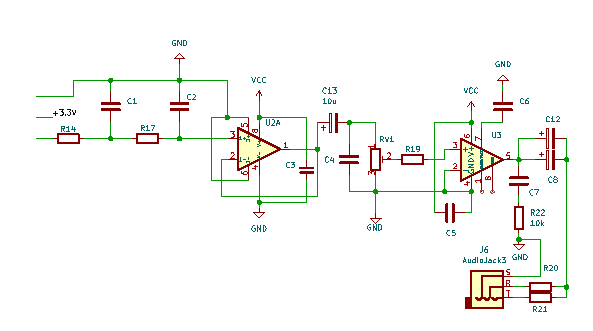
\includegraphics[width=\textwidth]{../../images/dac.pdf}
    \caption{Schéma analogové častí audio výstupu.}
    \label{fig:dac}
\end{figure}

Tato podkapitola popisuje analogovou část obvodu určenou pro filtraci a~zesílení audio signálu
generovaného mikrokontrolérem. Návrh vychází z~požadavku na převod
digitálně reprezentovaného signálu (PWM) na analogový průběh a~jeho následné zesílení na úroveň
vhodnou pro reprodukci, jak ilustruje schéma na obrázku~\ref{fig:dac}.

\subsection{Vstupní signál a~předzpracování}

Zvukový signál je generován mikrokontrolérem jako výstup emulovaného APU,
přičemž jednotlivé vzorky jsou reprezentovány digitální hodnotou. Tento signál je následně
převáděn na výstupní pin mikrokontroléru ve formě \textbf{PWM} (\textit{Pulse Width Modulation}),
který vzniká změnou střídy (\textit{duty cycle}) digitálního signálu na výstupním pinu, kde šířka pulzu
odpovídá amplitudě aktuálního audio vzorku. PWM signál obsahuje nízkofrekvenční
složku (audio) spolu s~vysokofrekvenční nosnou složkou danou frekvencí \SI{250}{\kilo\hertz}.

Běžná audio zařízení vyžadují spojitý analogový signál, který mikrokontrolér bez interního DA
převodníku nedokáže přímo generovat. Analogový průběh je proto aproximován v digitální doméně a
následně rekonstruován pomocí vnějších obvodů.

Za účelem získání analogového signálu je PWM výstup veden přes \textbf{pasivní dolní propust}
tvořenou rezistory R14, R17 a~kondenzátory C1, C2. Tento filtr realizuje aproximaci integrace PWM
signálu, čímž dochází k~potlačení vysokofrekvenčních složek a~zachování obálky signálu. Výsledný
signál je přiveden na neinvertující vstup operačního zesilovače U2A.

\subsection*{První zesilovací stupeň}

Operační zesilovač U2A je zapojen jako napěťový sledovač (buffer), který zároveň funguje jako
\textbf{aktivní dolní propust}. Toto zapojení plní několik klíčových funkcí:

\begin{itemize}
    \item Oddělení zdroje signálu (mikrokontroléru) od zátěže.
    \item Snížení výstupní impedance.
    \item Stabilizace signálu před dalším zpracováním.
\end{itemize}

Zpětnovazební síť definuje frekvenční charakteristiku tohoto stupně a~omezuje šířku pásma
zesilovače, čímž dochází k~dodatečné filtraci vysokofrekvenční složky PWM signálu. Tento krok je
kritický pro snížení šumu a~nežádoucích artefaktů. Na výstupu zesilovače je zařazen vazební
kondenzátor C13, který odstraňuje stejnosměrnou složku a~umožňuje přenos pouze střídavé části
signálu.

\subsection*{Řízení hlasitosti}

Za vazebním kondenzátorem následuje trimr RV1, který slouží jako pasivní dělič napětí
pro řízení amplitudy signálu (hlasitosti). Trimr je využit pro kalibraci úrovně signálu
a~není určen k~uživatelskému ovládání.

\subsection*{Druhý zesilovací stupeň}

Operační zesilovač U3 představuje hlavní výkonový stupeň analogové části (audio zesilovač LM386). Je
zapojen jako neinvertující zesilovač, přičemž jeho zesílení je určeno zpětnovazební sítí
tvořenou komponenty R22, C5 a~C7. Tato konfigurace umožňuje:

\begin{itemize}
    \item Dosažení vyšší amplitudy výstupního signálu.
    \item Částečnou kompenzaci frekvenční charakteristiky.
    \item Stabilizaci zesilovače při kapacitní zátěži.
\end{itemize}

Kondenzátor C6 slouží jako \textbf{blokovací (decoupling) kondenzátor} napájení a~potlačuje
rušení přicházející z~napájecí větve.

\subsection{Výstupní vazba a~připojení zátěže}

Výstupní signál je veden přes paralelně zapojené vazební kondenzátory C12 a~C8. Toto uspořádání
(typicky kombinace většího elektrolytického a~menšího keramického kondenzátoru) zajišťuje odstranění
DC složky a~přenos nízkých frekvencí, a~zároveň slouží k~efektivní filtraci vysokofrekvenčního
rušení díky nízkému ekvivalentnímu sériovému odporu (ESR) keramické varianty. Společně tak bezpečně
chrání připojené zařízení (např. sluchátka nebo externí zesilovač).

Audio výstup je realizován pomocí konektoru J6 (audio jack), kde výstupní kanál je veden
přes rezistory R20 a~R21. Tyto rezistory slouží jako:

\begin{itemize}
    \item ochrana proti zkratu,
    \item omezení výstupního proudu,
    \item přizpůsobení impedance.
\end{itemize}

Výsledný analogový výstup je tak vhodný pro přímé připojení sluchátek (32–600 \si{\ohm}) i
externích zesilovačů a splňuje požadavky na frekvenční rozsah 20 Hz – 20 kHz při dostatečné
dynamice.

\end{document}
